\chapter{Team 3 Agent Design}\label{team_3_agent_design}

\section{The Agent}\label{the_agent}
The agent is designed to show different combinations of behaviour depending on three variables we have used to define any agent: stubbornness, \cite{chun_2005},  morality, \cite{waller_2015}, and mood. These three variables, defined in a range of 0 to 100 will change as the agent encounters a series of scenarios, with its personality shifting as events unravel.  The value of the different variables will affect how the agent takes decisions and acts, all of which will be explained in the following pages. \par
%%ADD THE MAIN CODE!!!
As the main function from which all the functionality of the agent is bases we have the \texttt{func (a *CustomAgent3) Run()}. The agent follows then next steps:
\begin{enumerate}
    \item The agent starts by updating its personality variables at the beginning of each day calling the necessary function. 
    \item If the agent was just ‘born’ it will learn an initial value for the average food consumed. 
    \item In the case the agent has changed floors the personality variables are changed depending on the characteristics of the change. 
    \item In the case the platform is not empty the agent will eat, the quantity depending on \texttt{a.takeFoodCalculation()}.
    \item Finally the agent will read and send any messages it considers.
\end{enumerate}

\subsection{Agent knowledge}
Agent 3 will be able to remember facts in order to make decisions. The variables in their memory are:
\begin{enumerate}
    \item \texttt{floors []int}: stores the floors the agent has been in before. This information is used on reshuffles to set our mood. 
    \item \texttt{lastHp int}: stores the last recorded HP value. Currently used to check a new day has started.
    \item \texttt{friends map[uuid.UUID]float64}: the agent is aware of the people they have met during their time in the tower. We assigned the agents uuid with our affection for them. Affection range is 0-1 (0 = dislike, 1 = like). 
    \item \texttt{foodLastEaten food.FoodType}: stores food last eaten.
    \item \texttt{foodLastSeen food.FoodType}: stores food last seen in the platform
    \item \texttt{foodMovingAvg float64}: stores moving average of food consumed
    \item \texttt{agentAge int}: stores how old (in days) the agent is.
    \item \texttt{treatyProposed messages.Treaty}: stores whether we already have a treaty with the person above
    \item \texttt{reshuffleEst int}: stores our estimation of reshuffle
    \item \texttt{hpAbove int}: stores the HP our neighbour above last told us they had
    \item \texttt{hpBelow int}: stores the HP our neighbour below last told us they had
  \end{enumerate}

\subsection{Agent decisions}
Agent 3 will be able to take decisions when receiving messages or after signing treaties and store these until they eat. This information is used to symbolize a predetermined decision has been taken instead of “impulsively” eating food depending solely on our hunger and state of mind.
\begin{enumerate}
    \item \texttt{foodToEat int}: stores how much food we have decided to eat in the next eating period.
    \item \texttt{foodToLeave int}: how much food we have decided to leave. It is necessary in case we want to: E.g eat 6 food and leave at least 10 food but when the platform arrives we see that it has 13 food. Both statements cannot be fulfilled and so we must prioritise one.
\end{enumerate}

\subsection{Agent variables}
Agent 3 will act differently depending on three different variables that define them, which will give the agent different personalities.
\begin{enumerate}
    \item \texttt{stubbornness int}: defines the likelihood of the agent to read a message. E.g: Stubbornness = 20 means there is a 20\% chance that the agent will ignore the message.
    \item \texttt{morality int}: defines the willingness of the agent to help others, \cite{waller_2015}, in other words, how much you care about other agents in the tower. 
    \item \texttt{mood int}: defines how likely the agent is to do things, it will affect its decision-making process.
\end{enumerate}
For the purpose of this agent, we will define personality as the individual differences in characteristic patterns of thinking, feeling, and behaving, as defined by the American Psychology Association. The traits that define an agent's personality are mutable, making our agent adapt its personality depending on the circumstances. 

\subsection{Agent generation}
%%TODO: have to add the code snippet
The function generates a new agent by initializing its variables, knowledge and decisions. All knowledge and decisions are defined initially as empty except for our last HP, which is initialized as 100 (as all agents are). \par
The variables of our agent, which define the personality it has, are randomly allocated to generate different agents. All three variables are defined to be in the range 0 to 100. Therefore morality and mood are randomly allocated to a value between 0 and 100. To ensure our agent is not completely deaf from the start we limit the initial stubbornness to 75. This does not limit the agent once it starts interacting and taking decisions. Which means it could possibly end up with a stubbornness value of 100 if the situations it goes through are auspicious for it.

\subsection{Agent Strategy}
Our agent follows the following strategy depending on the three agent variables:
\begin{enumerate}
    \item When morality is high, agents are more willing to listen and obey other agents.
    \item When morality is low, agents are less willing to listen and choose to eat more than they would when they have high morality.
    \item When stubbornness is high, agents will be “deaf” to most messages and not react to them.
    \item When stubbornness is high, agents are more willing to listen to messages.
    \item When mood is high, the actions taken are beneficial for more people.
    \item When mood is low, the actions taken are more beneficial for ourselves.
\end{enumerate}

\section{Agents emotions}\label{agents_emotions}
The following functions act as helpers for the rest of the agent code, enabling changes in the agents variables and reactions due to the value of these variables, as well as reactions to friendships. 

\subsection{Read function}
\texttt{func (a *CustomAgent3) read() bool}: our agent's stubbornness will limit the amount of messages it might read and react to. Each time we receive a message we call the \texttt{read()} function. This function will take into account the current stubbornness of the agent and return if the message must be read, and reacted to, or just discarded. 
This function works by randomly generating a number between 0 and 100. If this number is higher to the current stubbornness the message is read, if not it will be discarded. 

\subsection{Friendship Function}
\begin{sloppypar} %%Gives style warning so this sloppypar solves it
\texttt{func (a *CustomAgent3) updateFriendship(friend uuid.UUID, change int)}: changes the value of the friendships using Q-Learning. Change is either -1 or 1. \par
\end{sloppypar}
In the case we encounter a new agent we record this new ‘friendship’ in our memory. From the start we have an initial opinion on the agent we have just met. As for now we just know about its existence, we predefine a friendship level depending on our current morality. To ensure we don’t create a huge predisposition of the agent to others we limit this range on initial impression to be between 0.4 and 0.6

\subsection{Mood, Morality and Stubbornness helper functions }
\texttt{func (a *CustomAgent3) changeInMood(pointsMin, pointsMax, direction int)}: Helper function to change the mood. There is an aspect of randomisation and the mood changes between pointsMin and pointsMax. Depending on the direction, 1 or -1, the mood will change in a positive or negative sense, increased or reduced. \par
\begin{sloppypar} %%Gives style warning so this sloppypar solves it
\texttt{func (a *CustomAgent3) changeInMorality(pointsMin, pointsMax, direction int)}: same as before but changes morality. \par
\end{sloppypar}
\texttt{func (a *CustomAgent3) changeInStubbornness(change, direction int)}: same as before but changes stubbornness. \par

\subsection{Changes to environment}
Changes to the environment will change the variables our agent is defined by. We have defined two possible environmental changes our agent will be affected by:
\begin{enumerate}
    \item A new day \texttt{func (a *CustomAgent3) changeNewDay()}: changes our morality and mood depending on our HP that morning. Changes depend on our current HP, which we have divided in four possible situations: 0-19, 20-39, 40-74 and 75-100.
    \item A change in the floor we are located (reshuffle) \texttt{func (a *CustomAgent3) changeNewFloor()}: a change in the floor we are at will make the mood of our agent to change accordingly. We have designed for 4 possible scenarios to happen: 
    \begin{enumerate}
        \item We arrive at the highest floor we have ever been to: we get a boost of moodas we should be able to eat more than any other time, our mood can change positively between 5 and 10 points.
        \item We arrive at a higher floor than before, but not the highest we have ever been: We are higher than before which is positive for us. As we could have done better our mood increases but less than in the previous scenario, our mood can change positively between 0 and 5 points.
        \item We have arrived at a lower floor than before, but we have been lower: Our situation is worse than before but it could have been even worse. We lose mood points, our mood can change negatively between 0 and 5 points.
        \item We have arrived at the lowest floor ever: We have never been in a worse situation and our agent will suffer a blow from this change. Our mood can be specially affected in this scenario, our morale can change negatively between 5 and 15 points.
    \end{enumerate}
    Each scenario can affect our agent in a different way. To make the scenario as realistic as possible we have added an element of randomness to the change in mood, depending on the range given on each of the scenarios. \par
    Inside the function we store our new floor in our knowledge, we restart the HP of our neighbors, we don’t know who they are, and call \texttt{a.reshuffleEstimator()}. \par
    \texttt{func (a *CustomAgent3) reshuffleEstimator()}: ensures we do not accept treaties longer than two times the reshuffle period so there are less chances a treaty kills us 
\end{enumerate}

\section{Treaties}\label{treaties}

\subsection{Handling a proposed treaty}
Each Team 3 agent contains variables mood, morality, stubbornness and friendship, which dictate how an agent will send and respond to messages, and how much food an agent will take from the platform. These variables are initialised differently for each agent, and evolve independently depending on the actions of that agent each tick. In order to engineer a system that can be self-organising, it is important to provide agents with the capability to agree to act together. This means that agents will commit to performing the same action when under the same circumstances. A treaty, which is used by all agent types and is explained previously, will need to define the circumstances, or condition, and the action, or request. Hence, the implementation is as follows: \par
Agents that are in a bad mood will not accept treaties that they need to honour even when they are at very low health, since they have a low confidence in the capabilities of other agents. However, when in a good mood agents will accept treaties that must be honoured even at low health. Morality is an indicator of the agent’s desire to perform actions that will benefit others, as opposed to just benefiting the agent itself. Therefore, very moral agents will accept treaties that involve them consuming just enough food to survive, but not too little food that they die or too much that they are too greedy. Similarly, very immoral agents will only accept treaties where they consume more than enough food, since they disregard the food needs of the other agents. The table below displays of the mood and morality values which agents must satisfy to accept treaties with any given condition on AgentPosition, and request of FoodTaken.\par
\begin{figure}[htb]
    \centering
    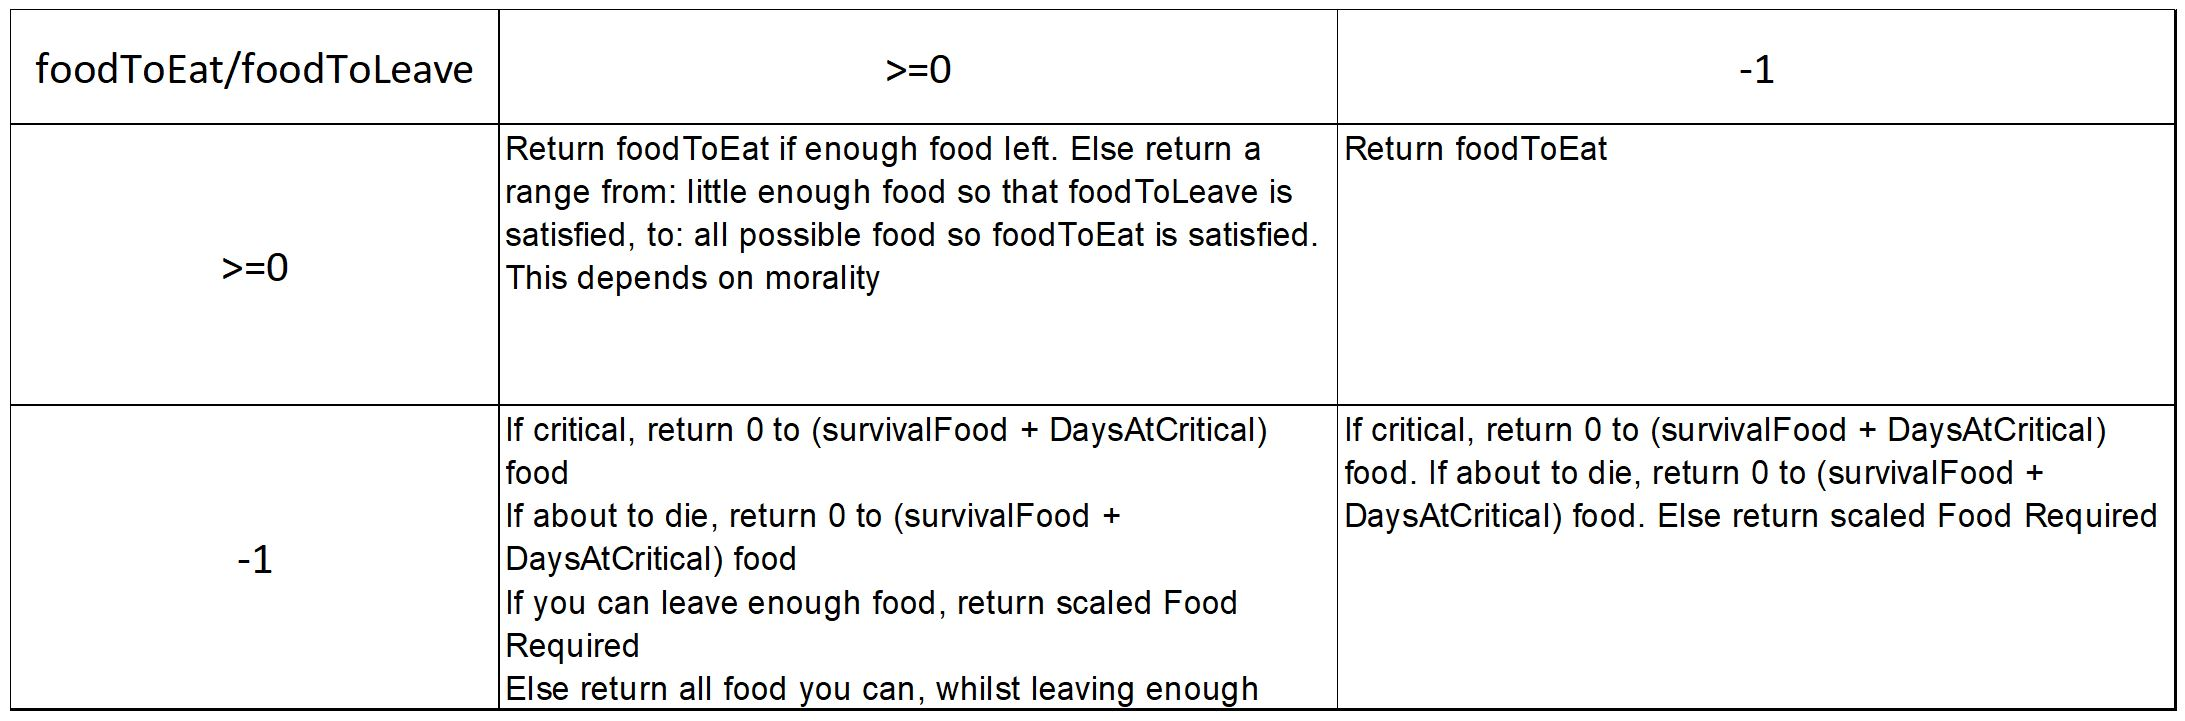
\includegraphics[width=1\linewidth]{005_team_3_agent_design/images/table1.jpg}
\end{figure}
Treaties also have a specified duration and signature count, which are visible to any agent that wishes to sign the treaty. These are likely to affect an agent’s decision to accept a treaty, and have been taken into account. If a treaty lasts longer than twice the reshuffle period, an agent deems it too far into the future to be able to predict what will happen, and plans to reject the treaty. However, if a treaty has more than five signatures, it is an extremely popular treaty. If the agent plans to reject the treaty as a result of any previous logic, the influence of peer pressure will cause the agent to reconsider accepting the treaty. The stubbornness of an agent is used as the likelihood to give in to peer pressure, so more stubborn agents are less likely to reconsider their response, and more likely to stick with their original decision.\par
After all of this, a boolean value to accept or reject the treaty is sent in a reply message, informing the proposed treaty sender of the agent’s decision to accept or reject the treaty.

\section{Agents Food}\label{agents_food}
The food calculation function first takes into account treaties which the agent in question has agreed to using the handleTreaties function, as by construction treaties take highest priority when deciding the variable foodToLeave, which is the amount of food an agent leaves on the platform. Therefore, when the agent in question has accepted a treaty the food calculations become dependent on the treaty conditions.\par
All treaties which the agent has accepted are gone through individually to calculate the final amount of food to take from the platform. For each treaty which is accepted by the respective agent, \texttt{conditionMet()} function checks whether the condition stated within the specific treaty is satisfied, in which case the agreed upon amount of food to leave on the platform is calculated and assigned to the foodToLeave variable, replacing its previous value. In the case where the treaty request is not to leave food on the platform, but to inform the sender of the treaty of our agent's HP, a foodToLeave is unchanged and instead a message containing our current HP is sent to the sender agent. After all the treaty conditions have been dealt with, we move onto the actual food calculation portion of the function.\par
The food calculation function calculates the amount of food an agent should take and leave on the platform depending on various variables, including morality, and if specified, foodToEat and foodToLeave. foodToEat and foodToLeave take the value “-1” if they are not defined by the end of  the message pipeline. This leads to four possible cases of foodToEat and foodToLeave values, which are handled differently. This logic is expressed in the following table:
\begin{figure}[htb]
    \centering
    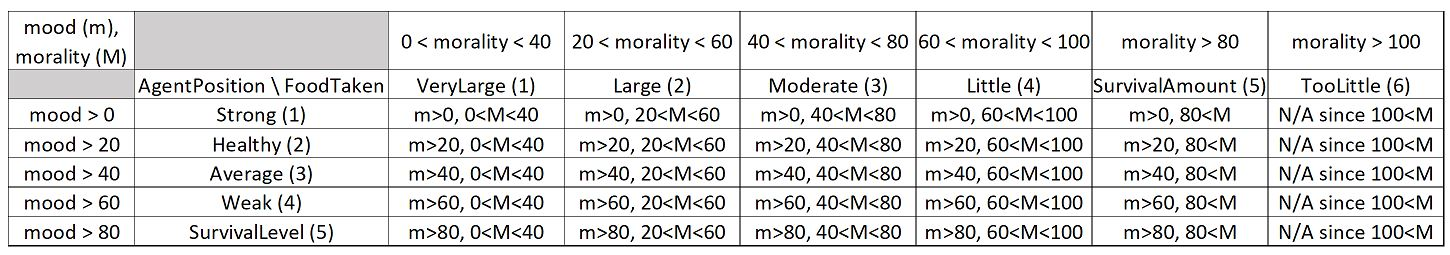
\includegraphics[width=1\linewidth]{005_team_3_agent_design/images/table2.jpg}
\end{figure}
Notice that when foodToEat is unspecified, the agent will automatically desire to eat at least survivalFood food if it is dying (meaning having been in critical state for 2 days). However, when foodToEat is specified, this cannot be overwritten. Here, there is also no case which avoids death, since that should have been prevented in the message pipeline if desired.\par
The calculation of the foodToLeave and foodToEat is scaled according to the current morality of the agent. When the morality of the agent is maximum (100), the agent will take the most considerate action with respect to the other agents. E.g. If food on the platform <= foodToLeave + foodToEat then the agent will opt to leave the requested amount of food instead of eating the desired amount of food. When the morality of the agent is at a minimum (0), the agent will take the most selfish action possible. Eg. If food on the platform <= foodToLeave + foodToEat then the agent will eat the amount of food they desire regardless of how much will be left on the platform afterwards.\par
A number of helper functions have been created to improve the readability of the code. These are explained below:
\begin{enumerate}
    \item \texttt{func (a *CustomAgent3) foodReqCalc(initalHP int, targetHP int) int}: based on the input initialHP and targetHP variables it calculates the amount of food which is required for the agent to reach its targetHP after the health update and decay processes which occur throughout a day in the tower. The formula is complex, and is reverse engineered using food parameters.
    \item \texttt{func (a *CustomAgent3) targetHPCalc() int}: calculates a reasonable targetHP for the agent to aim for based on its currentHP value. At lower HPs the agent should aim to gain more HP as they are in a weakened state and would like to become healthier. At a medium HP level (65 HP) the agent should aim to remain at that HP level. Finally, when at a high HP level the agent should aim to lose some HP as in a hostile environment such as the tower their conscience should not allow them to act so selfishly. This is done using a linear equation which scales the targetHP accordingly between 20HP (if HP=10) and 93HP (if HP=100), the minimum and maximum HP values excluding the critical state which behaves differently. Formula used: (9/11)*currentHP + 12.
    \item \texttt{func foodRange(metric int, min int, max int) int}: this function returns a value ranging between the min and max variables. The value returned is equal to max when the metric is 0, and min when the metric is 100. Formula used: max - metric / (100 / (max - min))
    \item \texttt{func foodScale(number int, metric int, minScale float, maxScale float) int}: this function returns a value ranging between number*minScale and number*maxScale based on the metric variable, which ranges from 0 to 100. Formula used: (number * minScale * metric) / 100 + number * maxScale * (100 - metric) / 100
\end{enumerate}

\section{Agents Messages}\label{agents_messages}